\documentclass[a4paper]{article}

\usepackage{inputenc}
\usepackage[british,UKenglish]{babel}
\usepackage{amsmath}
%\usepackage{titlesec}
\usepackage{color}
\usepackage{graphicx}
\usepackage{fancyref}
\usepackage{hyperref}
\usepackage{float}
\usepackage{scrextend}
\usepackage{setspace}
\usepackage{xargs}
\usepackage{multicol}
\usepackage{nameref}

\usepackage{sectsty}
\usepackage{multicol}
\usepackage{multirow}
\usepackage[procnames]{listings}
\usepackage{appendix}

\newcommand\tab[1][1cm]{\hspace*{#1}}
\hypersetup{colorlinks=true, linkcolor=black}
\interfootnotelinepenalty=10000

\newcommand{\cleancode}[1]{\begin{addmargin}[3em]{3em}\texttt{\textcolor{cleanOrange}{#1}}\end{addmargin}}
\newcommand{\cleanstyle}[1]{\text{\textcolor{cleanOrange}{\texttt{#1}}}}


\usepackage[colorinlistoftodos,prependcaption,textsize=footnotesize]{todonotes}
\newcommandx{\commred}[2][1=]{\textcolor{Red}
{\todo[linecolor=red,backgroundcolor=red!25,bordercolor=red,#1]{#2}}}
\newcommandx{\commblue}[2][1=]{\textcolor{Blue}
{\todo[linecolor=blue,backgroundcolor=blue!25,bordercolor=blue,#1]{#2}}}
\newcommandx{\commgreen}[2][1=]{\textcolor{OliveGreen}{\todo[linecolor=OliveGreen,backgroundcolor=OliveGreen!25,bordercolor=OliveGreen,#1]{#2}}}
\newcommandx{\commpurp}[2][1=]{\textcolor{Plum}{\todo[linecolor=Plum,backgroundcolor=Plum!25,bordercolor=Plum,#1]{#2}}}

\def\code#1{{\tt #1}}

\def\note#1{\noindent{\bf [Note: #1]}}

\makeatletter
%% The "\@seccntformat" command is an auxiliary command
%% (see pp. 26f. of 'The LaTeX Companion,' 2nd. ed.)
\def\@seccntformat#1{\@ifundefined{#1@cntformat}%
   {\csname the#1\endcsname\quad}  % default
   {\csname #1@cntformat\endcsname}% enable individual control
}
\let\oldappendix\appendix %% save current definition of \appendix
\renewcommand\appendix{%
    \oldappendix
    \newcommand{\section@cntformat}{\appendixname~\thesection\quad}
}
\makeatother


% "define" Scala
\usepackage[T1]{fontenc}  
\usepackage[scaled=0.82]{beramono}  
\usepackage{microtype} 

\sbox0{\small\ttfamily A}
\edef\mybasewidth{\the\wd0 }

\lstdefinelanguage{scala}{
  morekeywords={abstract,case,catch,class,def,%
    do,else,extends,false,final,finally,%
    for,if,implicit,import,match,mixin,%
    new,null,object,override,package,%
    private,protected,requires,return,sealed,%
    super,this,throw,trait,true,try,%
    type,val,var,while,with,yield},
  sensitive=true,
  morecomment=[l]{//},
  morecomment=[n]{/*}{*/},
  morestring=[b]",
  morestring=[b]',
  morestring=[b]"""
}

\usepackage{color}
\definecolor{dkgreen}{rgb}{0,0.6,0}
\definecolor{gray}{rgb}{0.5,0.5,0.5}
\definecolor{mauve}{rgb}{0.58,0,0.82}

% Default settings for code listings
\lstset{frame=tb,
  language=scala,
  aboveskip=3mm,
  belowskip=3mm,
  showstringspaces=false,
  columns=fixed, % basewidth=\mybasewidth,
  basicstyle={\small\ttfamily},
  numbers=none,
  numberstyle=\footnotesize\color{gray},
  % identifierstyle=\color{red},
  keywordstyle=\color{blue},
  commentstyle=\color{dkgreen},
  stringstyle=\color{mauve},
  frame=single,
  breaklines=true,
  breakatwhitespace=true,
  procnamekeys={def, val, var, class, trait, object, extends},
  procnamestyle=\ttfamily\color{red},
  tabsize=2
}

\lstnewenvironment{scala}[1][]
{\lstset{language=scala,#1}}
{}
\lstnewenvironment{cpp}[1][]
{\lstset{language=C++,#1}}
{}
\lstnewenvironment{bash}[1][]
{\lstset{language=bash,#1}}
{}
\lstnewenvironment{verilog}[1][]
{\lstset{language=verilog,#1}}
{}



%代码段设置
\lstset{numbers=left,
basicstyle=\tiny,
numberstyle=\tiny,
keywordstyle=\color{blue!70},
commentstyle=\color{red!50!green!50!blue!50},
frame=single, rulesepcolor=\color{red!20!green!20!blue!20},
escapeinside=``
}

\graphicspath{ {images/} }
\usepackage{ctex}
\usepackage{graphicx}
\usepackage{color,framed}%文本框
\usepackage{listings}
\usepackage{caption}
\usepackage{amssymb}
\usepackage{enumerate}
\usepackage{xcolor}
\usepackage{bm} 
\usepackage{lastpage}%获得总页数
\usepackage{fancyhdr}
\usepackage{tabularx}  
\usepackage{geometry}
\usepackage{minted}
\usepackage{graphics}
\usepackage{subfigure}
\usepackage{float}
\usepackage{pdfpages}
\usepackage{pgfplots}
\pgfplotsset{width=10cm,compat=1.9}
\usepackage{multirow}
\usepackage{footnote}
\usepackage{booktabs}

%-----------------------伪代码------------------
\usepackage{algorithm}  
\usepackage{algorithmicx}  
\usepackage{algpseudocode}  
\floatname{algorithm}{Algorithm}  
\renewcommand{\algorithmicrequire}{\textbf{Input:}}  
\renewcommand{\algorithmicensure}{\textbf{Output:}} 
\usepackage{lipsum}  
\makeatletter
\newenvironment{breakablealgorithm}
  {% \begin{breakablealgorithm}
  \begin{center}
     \refstepcounter{algorithm}% New algorithm
     \hrule height.8pt depth0pt \kern2pt% \@fs@pre for \@fs@ruled
     \renewcommand{\caption}[2][\relax]{% Make a new \caption
      {\raggedright\textbf{\ALG@name~\thealgorithm} ##2\par}%
      \ifx\relax##1\relax % #1 is \relax
         \addcontentsline{loa}{algorithm}{\protect\numberline{\thealgorithm}##2}%
      \else % #1 is not \relax
         \addcontentsline{loa}{algorithm}{\protect\numberline{\thealgorithm}##1}%
      \fi
      \kern2pt\hrule\kern2pt
     }
  }{% \end{breakablealgorithm}
     \kern2pt\hrule\relax% \@fs@post for \@fs@ruled
  \end{center}
  }
\makeatother
%------------------------代码-------------------
\usepackage{xcolor} 
\usepackage{listings} 
\lstset{ 
breaklines,%自动换行
basicstyle=\small,
escapeinside=``,
keywordstyle=\color{ blue!70} \bfseries,
commentstyle=\color{red!50!green!50!blue!50},% 
stringstyle=\ttfamily,% 
extendedchars=false,% 
linewidth=\textwidth,% 
numbers=left,% 
numberstyle=\tiny \color{blue!50},% 
frame=trbl% 
rulesepcolor= \color{ red!20!green!20!blue!20} 
}

%-------------------------页面边距--------------
\geometry{a4paper,left=2.3cm,right=2.3cm,top=2.7cm,bottom=2.7cm}
%-------------------------页眉页脚--------------
\usepackage{fancyhdr}
\pagestyle{fancy}
\lhead{\kaishu \leftmark}
% \chead{}
\rhead{\kaishu 并行程序设计实验报告}%加粗\bfseries 
\lfoot{}
\cfoot{\thepage}
\rfoot{}
\renewcommand{\headrulewidth}{0.1pt}  
\renewcommand{\footrulewidth}{0pt}%去掉横线
\newcommand{\HRule}{\rule{\linewidth}{0.5mm}}%标题横线
\newcommand{\HRulegrossa}{\rule{\linewidth}{1.2mm}}
\setlength{\textfloatsep}{10mm}%设置图片的前后间距
%--------------------文档内容--------------------

\begin{document}
\renewcommand{\contentsname}{目\ 录}
\renewcommand{\appendixname}{附录}
\renewcommand{\appendixpagename}{附录}
\renewcommand{\refname}{参考文献} 
\renewcommand{\figurename}{图}
\renewcommand{\tablename}{表}
\renewcommand{\today}{\number\year 年 \number\month 月 \number\day 日}

%-------------------------封面----------------
\begin{titlepage}
    \begin{center}
    
\includegraphics[width=0.8\textwidth]{NKU.png}\\[1cm]
    \vspace{20mm}
		\textbf{\huge\textbf{\kaishu{计算机学院}}}\\[0.5cm]
		\textbf{\huge{\kaishu{并行程序设计期末报告}}}\\[2.3cm]
		\textbf{\Huge\textbf{\kaishu{实验总结}}}

		\vspace{\fill}
    
    % \textbf{\Large \textbf{并行程序设计期末实验报告}}\\[0.8cm]
    % \HRule \\[0.9cm]
    % \HRule \\[2.0cm]
    \centering
    \textsc{\LARGE \kaishu{姓名\ :\ 王泽舜}}\\[0.5cm]
    \textsc{\LARGE \kaishu{学号\ :\ 2310655}}\\[0.5cm]
    \textsc{\LARGE \kaishu{专业\ :\ 计算机科学与技术}}\\[0.5cm]
    
    \vfill
    {\Large \today}
    \end{center}
\end{titlepage}

\renewcommand {\thefigure}{\thesection{}.\arabic{figure}}%图片按章标号
\renewcommand{\figurename}{图}
\renewcommand{\contentsname}{目录}  
\cfoot{\thepage\ of \pageref{LastPage}}%当前页 of 总页数
\clearpage
\tableofcontents
\newpage
\clearpage
\section{SIMD算法优化哈希部分}
\subsection{原算法原理}
MD5算法核心流程分为四个处理阶段(Round),每轮包含16次相似操作:
\begin{itemize}
  \item \textbf{消息填充}:将输入补足为512bit的整数倍(具体由StringProcess完成)
  \item \textbf{初始化}:初始化state[][],x[i],abcd
  \item \textbf{四轮处理}:共64步非线性运算
  \item \textbf{结果输出}:组合结果生成128位哈希值
  \end{itemize}
  

\subsection{改造点分析}
原始代码存在以下可并行化部分:

\begin{table}[h]
\centering
\begin{tabular}{lll}
\toprule
\textbf{文件} & \textbf{原始实现} & \textbf{改造内容} \\
\midrule
main.cpp & 单次处理1个口令 & 改为4口令批量处理 \\
md5.h & 标量位运算 & NEON向量化指令 \\
md5.cpp & 串行四轮运算 & SIMD并行四轮 \\
\bottomrule
\end{tabular}
\caption{代码改造对照表}
\end{table}

\subsection{关键技术实现}
\par 我们需要修改两部分,第一部分是核心的哈希函数的向量化,第二部分是中间变量修改为并行版本,这就需要回去找neon指令集的对应函数
\subsubsection{核心运算向量化}
采用ARM NEON intrinsics实现:

\begin{lstlisting}[language=C++,caption=FF函数的并行版本]
#define FF_NEON(a, b, c, d, x, s, ac) { \
    a = vaddq_u32(a, vaddq_u32( \
        vaddq_u32(F_NEON(b, c, d), x), ac)); \
    a = ROTATELEFT_NEON(a, s); \
    a = vaddq_u32(a, b); \
}
\end{lstlisting}

\subsubsection{消息块处理}
并行加载4个消息块,将ff等函数的七个参数全部向量化:
\begin{lstlisting}[language=C++,caption=同步修改了stringprocess函数,用以填充paddedMessage数组]
    paddedMessage = new Byte *[4]; 
    for (int i = 0; i < 4; i += 1) {
        paddedMessage[i] = StringProcess(inputs[i], &messageLength[i]);
    }

    \end{lstlisting}
    
    \begin{lstlisting}[language=C++,caption=加载一些中间变量]
            // 为4个并行哈希初始化MD5常量
            uint32_t initial_state[4][4] = {
                {0x67452301, 0x67452301, 0x67452301, 0x67452301}, 
               ......
            };
            // 复制到输出状态数组
            for (int i = 0; i < 4; ++i) {for (int j = 0; j < 4; ++j) {
                    state_neon[i][j] = initial_state[i][j];}}
            // 加载到NEON寄存器
            uint32x4_t a = vld1q_u32(state_neon[0]); 
            ......
            //并行加载原先的x[16],算法和组合方式照搬
           uint32x4_t x_neon[16];
    for (int i1 = 0; i1 < 16; i1++) {
        // 计算4个消息块用来初始化的四字节的地址
        Byte* msg0 = &paddedMessage[0][i*64 + i1 * 4];
        ......
        // 并行加载
        uint32x4_t x0 = vmovq_n_u32(msg0[0] | (msg1[0] << 8) | (msg2[0] << 16) | (msg3[0] << 24));
        ......  
        // 组合结果
        x_neon[i1] = vorrq_u32(
            vshlq_n_u32(x3, 24),
            vorrq_u32(vshlq_n_u32(x2, 16),
            vorrq_u32(vshlq_n_u32(x1, 8),x0)));}
    \end{lstlisting}

\begin{lstlisting}[language=C++,caption=hash函数具体执行示例]
    // sx和立即数也都向量化
    FF_NEON(a, b, c, d, x_neon[0], vdupq_n_u32(s11), vdupq_n_u32(0xd76aa478));
    ......
\end{lstlisting}
\par 优化后的哈希时长在总指令量为1000w的情况下从3.00787s优化到了2.36285s,加速比为1.27x。
\par 本次实验中,主要改进在于将原有的标量位运算改为向量化处理,利用NEON指令集实现了FF、GG等函数的并行化。通过对消息块的并行加载和处理,显著提升了MD5算法的执行效率。
\par 而并不涉及修改算法,主要工作量在于理清和维持中间量的传递关系,还有去查neon指令集的官方文档找替换函数

\section{多线程并行化实验}
本实验要改进的核心算法本质是在密码猜测过程中,对PT(猜测模板)的最后一个segment进行具体的填充。以$L_8D_2$为例,经过前序优先队列的初始化和不断迭代,$L_8$部分已被实例化,剩余的$D_2$需要在此处补全。假设模型统计得到12、11、23这三个具体的值,则本循环会依次将这三个值填充到$D_2$,从而生成三个新的口令猜测。

该过程在代码中表现为如下循环:

\begin{lstlisting}[caption=核心循环伪代码]
for (int i = 0; i < pt.max_indices[0]; i += 1) {
    string guess = a->ordered_values[i];
    guesses.emplace_back(guess);
    total_guesses += 1;
}
\end{lstlisting}
\par 考虑并行化上述循环,当我们将上述任务划分成多线程时,基本地,需要考虑以下几点:
\par 1.如果是静态的分配任务,分到最后剩余的部分很可能少于线程数,这时需要考虑如何处理剩余任务。我们在代码中\texttt{int num\_threads = std::min(4, n);}来避免上述情况
\par 2.多个线程需要访问共享数据(如guesses),如何确保数据的一致性和线程安全:我们考虑提前将guesses数组扩容到目标大小,每个线程负责写入自己负责的区间,这样在保证安全的同时也避免了更多的分配内存操作。。
% \par 3.任务划分:如何将循环中的任务均匀分配给多个线程,以充分利用多核CPU的计算能力
% \par 4.负载均衡:如何动态调整各个线程的工作量,以避免某些线程过载而其他线程空闲的情况。
\par 3.如果只考虑将这个循环并行化,由于任务粒度太细,可能创建销毁线程的开销大于优化的收益,因此可以尝试PT层面的并行
\subsection{for循环并行优化代码分析}
\subsubsection{基于pthread的并行优化实现}
\begin{lstlisting}[caption=pthread并行实现关键代码片段]
struct ThreadArg2 {
    segment* a;
    std::string guess_prefix;
    int start, end;
    std::vector<std::string>* guesses_ptr;
    int offset;
};
//我们将前缀和指针、偏移量传入线程函数中,在内部计算要写入结果的位置
// 线程函数
void* thread_func2(void* arg) {
    ThreadArg2* t_arg = (ThreadArg2*)arg;
    for(int i = t_arg->start; i < t_arg->end; ++i) {
        (*t_arg->guesses_ptr)[t_arg->offset + (i - t_arg->start)] = 
            t_arg->guess_prefix + t_arg->a->ordered_values[i];
    }
    return nullptr;
}

// 主线程分配任务
int n = pt.max_indices[pt.content.size() - 1];
int num_threads = std::min(4, n);//处理剩余量
size_t old_size = guesses.size();
guesses.resize(old_size + n);//结果扩容
......
for(int t = 0; t < num_threads; ++t) {
   .....//创建线程
}
for(int t = 0; t < num_threads; ++t) {
    if(args[t].start < args[t].end)
        pthread_join(threads[t], nullptr);}
total_guesses += n;
\end{lstlisting}

\subsubsection{总结}
\par 通过pthread并行优化,PCFG口令生成算法在多核环境下能显著提升生成速度,尤其适合大规模口令空间的遍历任务。优化后的实现既保证了线程安全,又减少了内存分配和拷贝的开销,是高效并行编程的典型范例。
\par 基础实验的主要工作量是熟悉pthread的代码格式,同时在前期改代码但难以实现加速的过程中也让我对计算、分配内存、线程开销等成本有一定意识,最后通过优化减少分配内存次数实现了加速。
\subsection{OpenMP并行化设计思路与代码实现对比分析}
\textbf{OpenMP并行化设计思路:}
为消除多线程竞争和提升效率,采用如下并行化策略:
\begin{itemize}
    \item \textbf{空间预分配}:先由主线程(或\#pragma omp single)将guesses扩展到最终所需大小,记录插入起始下标。
    
    \item \textbf{分段并行写入}:用\#pragma omp parallel for,每个线程写自己负责的区间,避免push\_back带来的锁竞争。
    
    \item \textbf{总数累加优化}:total\_guesses只需在并行循环后由主线程统一加上本轮生成的数量。
\end{itemize}

\begin{lstlisting}[caption=OpenMP并行实现关键代码]
int n = pt.max_indices[pt.content.size() - 1];
int start_idx;//计算插入起始下标
#pragma omp single
{
    start_idx = guesses.size();
    guesses.resize(start_idx + n);
}
#pragma omp parallel for
for(int i = 0; i < n; ++i) {
    guesses[start_idx + i] = guess + a->ordered_values[i];
}
#pragma omp single
{
    total_guesses += n;
}
\end{lstlisting}
\section{MPI多进程并行化设计与实现}
为了将这个串行的过程在可接受的非严格pt概率序下并行化,采用MPI实现多进程并行。主要思路如下:
\begin{figure}[H] % [H]参数强制图片出现在这里
    \centering
    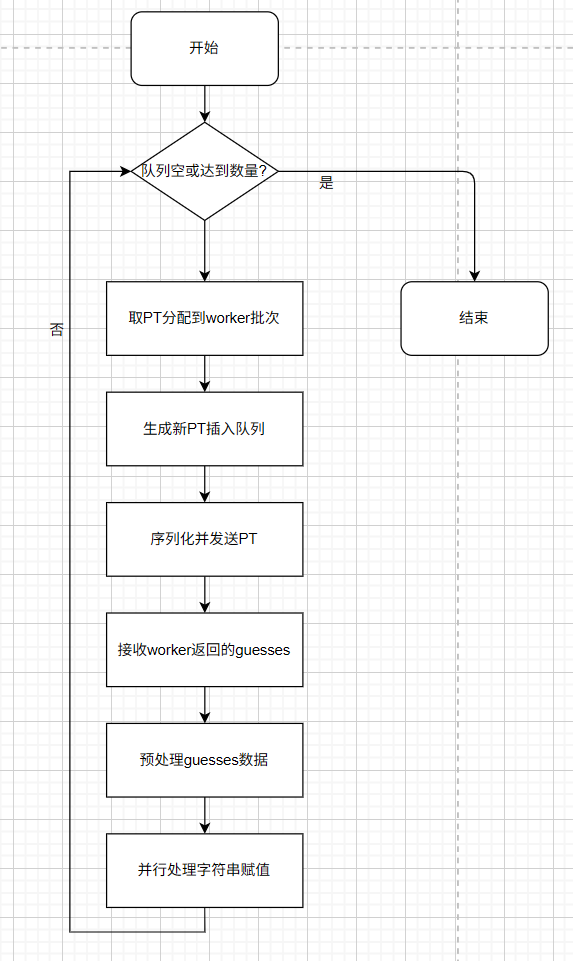
\includegraphics[width=0.8\textwidth]{image.png}
    \caption{MPI并行密码生成流程示意图}
    \label{fig:password_flow}
\end{figure}
如图\ref{fig:password_flow}所示,该流程主要包含以下步骤:
\begin{enumerate}
    \item \textbf{主进程(rank 0)} 负责PT任务分发和结果收集,以及原来的优先队列维护。
    \item \textbf{Worker进程(rank > 0)} 每次接收一批PT,批量generate guesses并返回主进程(原先的popnext的事主进程做,worker只generate PT)。
    \item \textbf{任务分发}:主进程每轮从优先队列顶部取出k*batch个pt,分发给各worker。
    \item \textbf{结果统计}:每个PT生成的guesses会发回主进程,主进程将结果重新生成成字符串再赋值给guesses的对应位置。
\end{enumerate}
更细致的解释见代码及注释:
\textbf{主流程核心代码与具体思路分析}如下:
\begin{lstlisting}[language=C++, caption={MPI并行密码生成算法核心代码}]
while (!q.priority.empty() && pt_idx < k * batch_size) {
    // 1. 从优先队列中取出batch_size个PT
    worker_batches[pt_idx % k].push_back(q.priority.front());
    
    // 2. 按照popNext()的逻辑生成PT并插入到优先队列
    vector<PT> new_pts = q.priority.front().NewPTs();
    for (PT pt : new_pts) {
        // ... 照抄popNext()代码,除了generate guesses的部分
    }
    
    // 3. 序列化PT并发送给worker
    for (int j = 0; j < batch_cnt; ++j) {
        std::string pt_str = serialize_PT(worker_batches[i][j]);
        int len = pt_str.size();
        MPI_Send(&len, 1, MPI_INT, i + 1, 0, MPI_COMM_WORLD);
        MPI_Send(pt_str.data(), len, MPI_CHAR, i + 1, 0, MPI_COMM_WORLD);
    }
    
    // 4.接收worker返回的guesses,生成字符串并插入到guesses
    // 4.1 接收数据
    MPI_Recv(&total_guess_count, 1, MPI_INT, i + 1, 0, MPI_COMM_WORLD, MPI_STATUS_IGNORE);
    std::vector<char> buf(total_guess_count * 64);
    MPI_Recv(buf.data(), total_guess_count * 64, MPI_CHAR, i + 1, 0, MPI_COMM_WORLD, MPI_STATUS_IGNORE);
    
    // 4.2 处理guesses
    // 预计算所有字符串长度和总字符数,以便接下来算每个guess字符串的位置
    std::vector<size_t> lengths(total_guess_count);
    for (int j = 0; j < total_guess_count; ++j) {
        lengths[j] = strnlen(buf.data() + j * 64, 64);
    }
    
    // 优化push_back:直接resize为原先长度+worker返回长度后
    //将缓冲区中计算好位置的字符串赋值给结果
    //基本mpi框架搭起来之后这部分一直是性能瓶颈
    //虽然改到现在这种方法但也没有做到加速
    size_t old_size = q.guesses.size();
    q.guesses.resize(old_size + total_guess_count);
    
    // 并行处理字符串赋值
    #pragma omp parallel for
    for (int j = 0; j < total_guess_count; ++j) {
        q.guesses[old_size + j].assign(buf.data() + j * 64, lengths[j]);
    }
    
    pt_idx++;
}
\end{lstlisting}
\textbf{Worker进程}:
基本上就是收批次长度、一批pt,反序列化,generate,然后返回guesses给主进程。

\subsection{并行算法性能分析与瓶颈诊断}
\begin{table}[htbp]
\centering
\caption{不同算法生成3000wguesses的时间性能对比(单位:秒)}
\label{tab:performance}
\begin{tabular}{lrrrrrr}
\hline
版本类型 & 测试次数 & \multicolumn{1}{c}{平均猜测时间} & \multicolumn{1}{c}{猜测时间标准差} & \multicolumn{1}{c}{平均哈希时间} & \multicolumn{1}{c}{平均训练时间} & \multicolumn{1}{c}{MPI通信占比} \\ \hline
带分块计时MPI & 10 & 3.58 & 2.87 & 11.35 & 18.47 & 68.7\% \\
无分块计时MPI & 10 & 3.34 & 0.42 & 9.31 & 14.95 & - \\
原始串行 & 10 & 1.28 & 0.30 & 8.15 & 15.59 & - \\ \hline
\end{tabular}
\end{table}




\begin{table}[h]
\centering
\caption{Performance Metrics Across Runs}
\small
\begin{tabular}{ccccccccc}
\toprule
Run & Guess Time (s) & \multicolumn{3}{c}{Deserialization Time (s)} & MPI Send Time (s) & \multicolumn{3}{c}{MPI Receive Time (s)} \\
\cmidrule(lr){3-5} \cmidrule(lr){7-9}
 & & Worker 1 & Worker 2 & Worker 3 & & Total & Pure Receive & Data Processing \\
\midrule
1 & 2.84876 & 0.0109539 & 0.0008191 & 0.0104925 & 0 & 2.35637 & 1.66293 & 0.639313 \\
2 & 8.95342 & 0.0157132 & 0.0278985 & 0.0238563 & 0.015377 & 7.38819 & 4.73557 & 2.35069 \\
3 & 11.5527 & 0.0186231 & 0.0079665 & 0.0317148 & 0.039071 & 9.88056 & 7.18948 & 2.40118 \\
4 & 8.47527 & 0.0209938 & 0.0056679 & 0.0165048 & 0.016278 & 7.45988 & 5.65764 & 1.56891 \\
5 & 4.07106 & 0 & 0.0116256 & 0 & 0.028064 & 3.19623 & 2.14647 & 0.927773 \\
6 & 3.61226 & 0.0005115 & 0.0044082 & 0.0007496 & 0.012729 & 2.88957 & 1.98154 & 0.822191 \\
7 & 3.65355 & 0.003308 & 0.0047705 & 0.0048067 & 0.014032 & 2.99156 & 2.03329 & 0.833825 \\
8 & 3.46606 & 0.0040221 & 0.0108211 & 0.0056186 & 0.009239 & 2.83929 & 1.94573 & 0.796273 \\
9 & 3.51646 & 0.0033345 & 0.0134644 & 0.0021544 & 0.011614 & 2.87988 & 1.92751 & 0.820323 \\
10 & 3.34775 & 0.0112826 & 0.0164895 & 0.0165029 & 0.015583 & 2.69302 & 1.83096 & 0.739929 \\
\midrule
\text{Avg.} & 5.3497 & 0.0089 & 0.0110 & 0.0112 & 0.0161 & 4.4575 & 3.1114 & 1.1842 \\
\bottomrule
\end{tabular}
\end{table}
\par 其中主要性能瓶颈为主进程接收字符串,更细分之后其中接收和处理基本七三开,接收阶段的瓶颈可能是子进程导致的,但数据显示子进程的反序列化并不费时间,其他操作和串行相同。而字符串处理见第三节中,已经尝试在算法层面进行优化,但仍然开销很大。
\par 后续做期末报告时候想到可以通过增加进程数来判断是不是任务分配不均导致完成时间方差太大,因此接收时间长,如果是这个原因的话,进程数增加会显著导致同一批workers个任务的接收卡壳时间进一步增长。
\begin{figure}[H] % [H]参数强制图片出现在这里
    \centering
    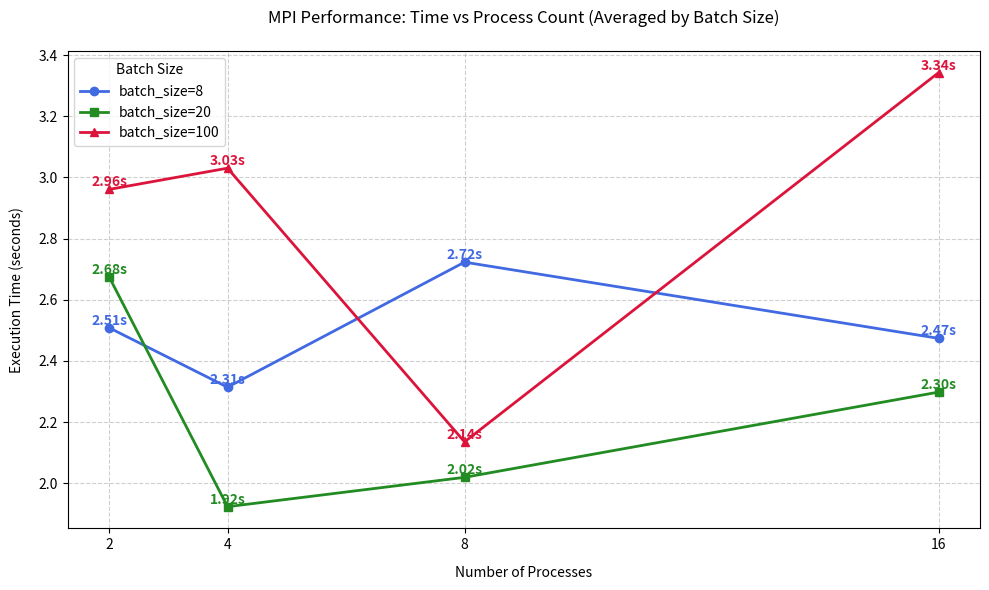
\includegraphics[width=0.8\textwidth]{table1.png}
    \caption{MPI并行密码生成流程示意图}
    \label{fig:test1}
\end{figure}

\par 如图\ref{fig:test1}所示,选取的每批pt数在20左右最优,进程数为4最优。同时结果显示进程数增加确实会导致结果更不稳定,时间也略微增长,于是我们考虑在发送PT之前,根据PT要操作的那个segment的indice大小来当做任务量,均衡每个worker的任务量,来避免一个worker任务很重卡住所有worker被主进程接收这种情况。
\textbf{关键修改如下:}
\begin{lstlisting}[language=C++,caption={基于工作量的PT负载均衡分配}]
std::vector<std::vector<PT>> worker_batches(k);
std::vector<size_t> worker_loads(k, 0); // 每个worker当前总工作量
int pt_idx = 0;
while (!q.priority.empty() && pt_idx < k * batch_size) {
    PT curr_pt = q.priority.front();
    // 计算PT的工作量
    size_t weight = 1;
    if (curr_pt.content.size() == 1) {
        weight = curr_pt.max_indices[0];
    } else {
        weight = curr_pt.max_indices[curr_pt.content.size() - 1];
    }
    // 找到当前负载最小的worker
    int min_worker = 0;
    for (int w = 1; w < k; ++w) {
        if (worker_loads[w] < worker_loads[min_worker]) min_worker = w;
    }
    worker_batches[min_worker].push_back(curr_pt);
    worker_loads[min_worker] += weight;

    // 生成新PT并插入优先队列(略)
    // ...
    q.priority.erase(q.priority.begin());
    pt_idx++;
}
\end{lstlisting}
\begin{table}[H]
\centering
\caption{均衡负载后生成3000万guesses的 Guess/Hash/Train 时间(单位:秒)}
\begin{tabular}{ccc}
\toprule
Guess Time & Hash Time & Train Time \\
\midrule
2.06185 & 4.93675 & 9.77798 \\
2.29269 & 5.54244 & 9.95582 \\
2.09226 & 4.59964 & 9.71931 \\
1.99932 & 4.56900 & 9.69441 \\
2.12546 & 5.03927 & 10.14700 \\
\bottomrule
\end{tabular}
\end{table}
\par 结果显示,在任务分配均衡的情况下,接收时间和处理时间的方差都显著降低,不再出现之前偶尔会跑到11s的情况。平均接收时间也有所下降,但仍然是整体性能瓶颈。
\subsection{总结}
\par 本实验通过MPI实现了PCFG口令猜测框架的高效多进程并行,主进程批量分发PT任务,worker并行生成guesses并返回,支持每个PT生成量的统计与分析。针对PT任务“重量”极不均衡的问题,采用动态、细粒度(具体到每个PT)的任务分配策略,以充分发挥并行计算资源,提高整体效率。

\section{CUDA并行基础要求设计与实现}
\textbf{优化思路}
\par 考虑字符串写入\texttt{guesses}这个过程,是否可以先将\texttt{guesses.resize(old\_size2 + pt.max\_indices[pt.content.size() - 1]\,\text{or}\,[0]);}得到的结果传入\texttt{cuda\_generate}函数,避免回收结果之后还得\texttt{emplace\_back}。然后发挥GPU对简单运算的优势,挨个把要赋值的值写入\texttt{guesses}中。
\par 但是这个过程无法实现,其一是GPU无法操作string指针,其二是即使我们采用char**存放,共享显存(一般为48kb)也放不下guesses那么大的块。因此我们退而求其次,
\par 考虑将所有后缀前缀拼接的过程放在GPU上进行。并在优化过程中,我们发现用二维数组存放所有的value会导致访存的不连续,导致性能下降,因此我们将二维数组扁平化为一维\texttt{char*}数组,使用\texttt{flat\_values}存放所有的value。GPU端每个线程负责将一个value拼接前缀(前缀是一维的,不用修改)之后写入计算好的区间。经测试,比原始实现:传二维\texttt{char**}数组(230s/50w guesses)优化到(1.85s/1000w guesses)。
\par 在做期末报告时,我们进行了更细致的分段计时,注意到预处理中分配内存的时间占用了约0.4s,检查代码发现我们在主机端为存放ordered\_values时候分配数组是在for循环中对每个value进行的,改为计算好总长度后一次性分配可以节省0.3s的时间,在改进之后我们提升到了(1.26s/1000w猜测)。
\par 以下是具体的实现代码,分为预处理及其优化,分配和拷贝内存,调用核函数,收集结果
\begin{lstlisting}[language=C++, caption={CUDA并行口令猜测核心流程}]
// 1. 主机端将所有value拼接为连续数组
int n = pt.max_indices[pt.content.size() - 1];
char **h_values = new char*[n];
        for (int i = 0; i < n; ++i) {
            h_values[i] = new char[value_len+1];
            strcpy(h_values[i], a->ordered_values[i].c_str());
        }
//在期末报告中改进为:
char *flat_values = new char[n * (value_len + 1)];
        for (int i = 0; i < n; ++i) {
            memcpy(flat_values + i * (value_len + 1), a->ordered_values[i].c_str(), value_len + 1);
        }
// 2. 分配device内存并拷贝数据
cudaMalloc(&d_result_data, n * (prefix_len + value_len + 1) * sizeof(char));
// 3. 启动核函数并行拼接
int block = 256;
int grid = (n + block - 1) / block;
generate_guesses_kernel_flat<<<grid, block>>>(d_flat_values, value_len, d_guess_prefix, prefix_len, d_result_data, n);
cudaDeviceSynchronize();
//核函数:(主要工作量是计算下标)
__global__ void generate_guesses_kernel_flat(const char *flat_values, int value_len, const char *d_guess_prefix, int prefix_len, char *result_data, int n) {
    int idx = blockIdx.x * blockDim.x + threadIdx.x;
    if (idx < n) {
        char *dst = result_data + idx * (prefix_len + value_len + 1);
        if (prefix_len > 0) {//如果是第二种情况,则将前缀也写到结果中
            for (int i = 0; i < prefix_len; ++i) dst[i] = d_guess_prefix[i];
        }
        const char *src = flat_values + idx * (value_len + 1);
        for (int i = 0; i < value_len; ++i) dst[prefix_len + i] = src[i];
        dst[prefix_len + value_len] = '\0';
    }
}
// 4. 回传结果
cudaMemcpy(result_data, d_result_data, n * (prefix_len + value_len + 1) * sizeof(char), cudaMemcpyDeviceToHost);
for (int i = 0; i < n; ++i) {
    guesses[offset + i].assign(result_data + i * (prefix_len + value_len + 1));
}
// 5. 释放内存
// ...
\end{lstlisting}
\textbf{cuda函数设计:}

\texttt{cuda\_generate\_guesses(char **h\_values, int value\_len, char *h\_guess\_prefix, int prefix\_len, int n, std::vector<std::string> \&guesses, size\_t offset)}
    \begin{itemize}
        %各参数解释
        \item \texttt{h\_values}:主机端的值数组
        \item \texttt{value\_len}:值长度
        \item \texttt{h\_guess\_prefix}:主机端的前缀,如果是第二个for循环就需要传入
        \item \texttt{prefix\_len}:前缀长度
        \item \texttt{n}:需要拼接的猜测数量
        \item \texttt{guesses}:拼接结果,直接用引用把guesses传进去
        \item \texttt{offset}:结果偏移量,因为传入的\texttt{guesses}有之前的结果,所以需要偏移到本次generate开始时候的位置,故用\texttt{size\_t old\_size = guesses.size();}赋值
    \end{itemize}
\par 核函数代码流程:根据是否有前缀,计算出每个线程需要处理的值的索引,和要写入结果数组的位置,然后将对应的值和前缀起来,写入结果数组中。
\subsection{cuda并行化实验总结}
\par 本次实验中,我们认识了如何用cuda编程对简单计算密集型的任务进行并行处理,相比多线程,cuda能够更细致地控制内存分配和数据传输,充分利用GPU的并行计算能力。
\par 同时我们也对内存分配,访存优化等更底层的优化空间有了一定了解。
\section{总结}
\par 本学期的并行实验中,我们从simd编程通过指令替代来优化和openMP练手开始,在pthread和MPI中通过亲自操作,学到了线程安全性如何保证,线程任务负载如何均衡。在cuda中更深入地体会到内存访问机制的巨大优化空间。在学习这些并行化代码结构的同时,也对程序从编译到运行整个过程中开销所在有了一定的认识。知道了有什么办法去探测、优化这些开销。
\par 期末所做的新内容为,mpi中测试batch值和进程数对性能的影响,均衡任务负载减小方差,cuda编程中优化内存分配
\end{document}